\documentclass[hidelinks,a4paper,12pt]{article}
\usepackage[left=2in, right=1in, top=1in, bottom=1in]{geometry}
\usepackage[table]{xcolor}
\usepackage{graphicx}
\usepackage{sectsty} %to customise headings
%\usepackage{attachfile}
%\usepackage{navigator}
\usepackage{times} %this is for the selection of font
%\usepackage[english]{babel} %this is for the selection of font
%\usepackage{Palatino}
%\usepackage{courier}
%\usepackage[T1]{fontenc}
%\renewcommand*\familydefault{\ttdefault} %% Only if the base font of the document is to be typewriter style
\usepackage{float}
\usepackage{fancyhdr}	
\usepackage[ampersand]{easylist}
\usepackage{amssymb}
\usepackage{enumitem}	
\usepackage{caption} \captionsetup[table]{singlelinecheck=false, margin=1em}
%\usepackage{tabu}
\usepackage{longtable}
\usepackage{booktabs}
\usepackage{eso-pic}
%\usepackage{transparent}
\usepackage{pdfpages}

\usepackage{ltablex}
\setlength{\LTpre}{0pt}
\setlength{\LTpost}{-15pt}

\usepackage{array}
\usepackage{tabularx}


\usepackage{pgfplots, pgfplotstable}
%\usepackage{makecell}
\usetikzlibrary{backgrounds}
% background color definition from pgfmanual-en-macros.tex
\definecolor{graphicbackground}{cmyk}{0,0,0,.03}
% key to change color
\pgfkeys{/tikz/.cd,
	background color/.initial=graphicbackground,
	background color/.get=\backcol,
	background color/.store in=\backcol,
}
\tikzset{background rectangle/.style={
		fill=\backcol,
	},
	use background/.style={    
		show background rectangle
	}
}
	
\pagestyle{fancy}
\fancyhf{}
\lhead{Project Synopsis}
\rhead{\textbf { \textsl{Service Request to a Cloud}}}
\lfoot{\scriptsize{MCS-44 Mini Project\\IGNOU Enrollment ID : 137132696\\ }}
% Set the right side of the footer to be the page number
\cfoot{}

\renewcommand{\headrulewidth}{0.4pt}
\renewcommand{\footrulewidth}{0.4pt}

%\usepackage{lipsum}% Used for dummy text.

\definecolor{titlepagecolor}{cmyk}{1,.60,0,.40}
\definecolor{namecolor}{cmyk}{0.4,.2,0.,.10} 
\definecolor{levelfirst}{cmyk}{0,0,0,0.70}
\definecolor{levelSecond}{cmyk}{1,.50,0,.10}
\definecolor{levelthird}{cmyk}{1,.50,0,.10}
\definecolor{levelfourth}{cmyk}{1,.50,0,.10}
\definecolor{levelfifth}{cmyk}{1,.50,0,.10}

\definecolor{tablecell1}{cmyk}{0.07,0.03,0.03,0.07}
\definecolor{tablecell2}{cmyk}{0.04,0.02,0.02,0.04}

\sectionfont{\fontsize{16}{22}\selectfont}
\subsectionfont{\fontsize{14}{18}\selectfont}
\subsubsectionfont{\fontsize{12}{16}\selectfont}
%\renewcommand{\abstractnamefont}{\fontsize{16}{22}\selectfont \bfseries}
%\renewcommand{\abstracttextfont}{\normalfont}

%-----------------------------------------------------------------
\begin{document}

\begin{titlepage}

\thispagestyle{empty}
\pagenumbering{roman}

\vspace{0.25in}
\hspace{-1.5in}
\includegraphics[ width={0.68\paperwidth} , keepaspectratio ]{Titlepage1.ps} \\
\vfill
\end{titlepage}
	
\newpage
\pagestyle{plain}
\pagenumbering{roman}
\setcounter{page}{2}

\hspace{-1.5in}
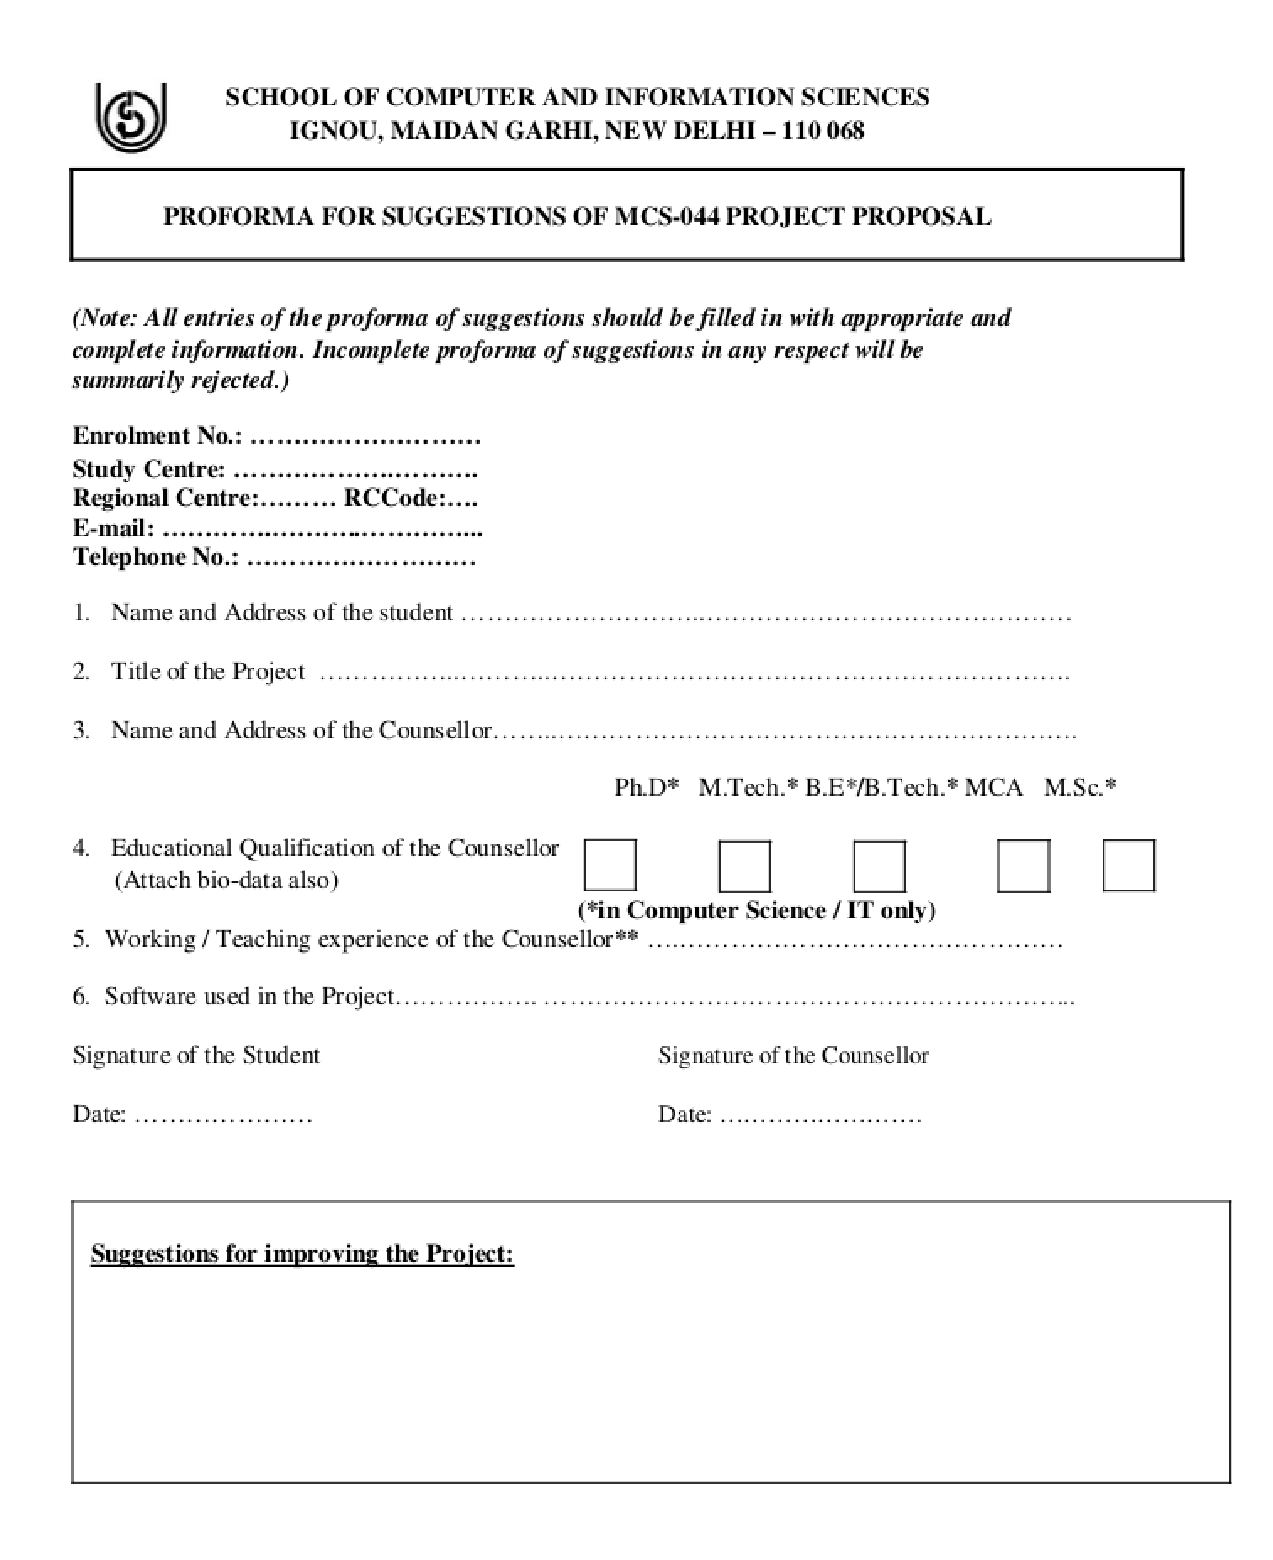
\includegraphics[ width={0.7\paperwidth} , keepaspectratio ]{pg2.eps} \\
\vfill

\newpage

\begin{center}
\hspace{-1.5in}
\textbf {CERTIFICATION} \\
\end{center}

\hspace{-1.5in}
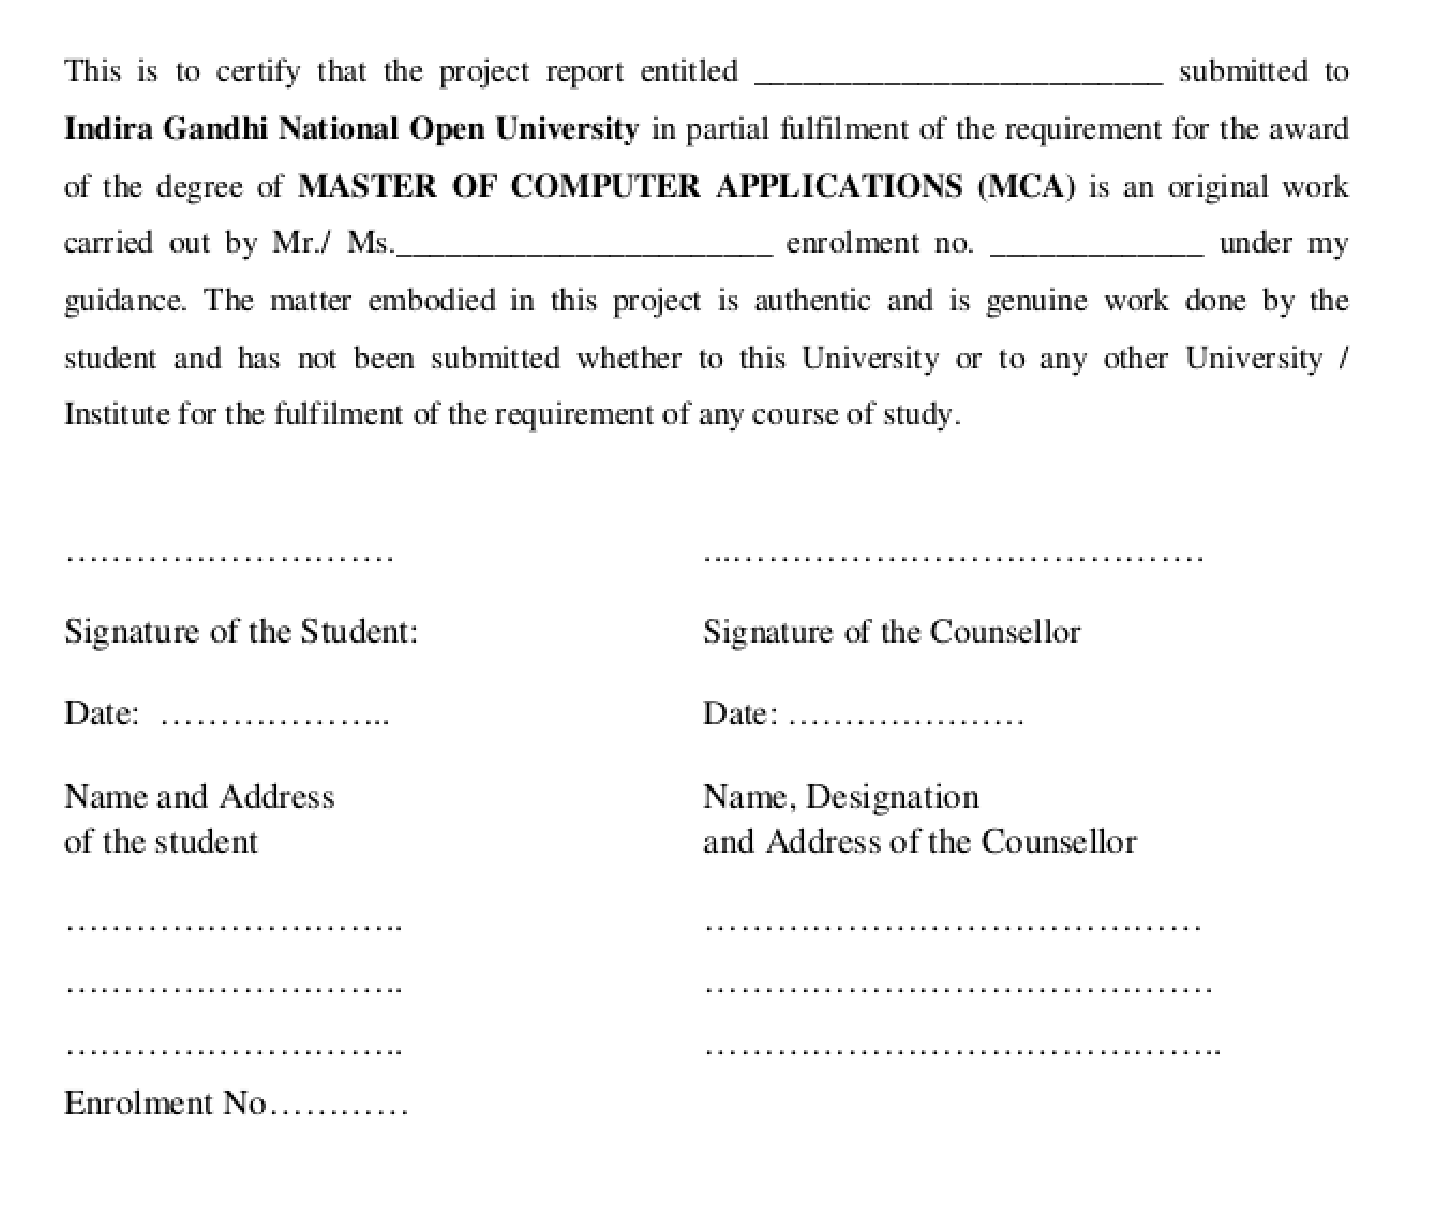
\includegraphics[ width={0.7\paperwidth} , keepaspectratio ]{pg3.eps}\\
\vfill

\newpage
	
\tableofcontents
	
\setcounter{tocdepth}{3}
	
	
\newpage

\clearpage

\pagestyle{plain}
\setcounter{page}{1}
\pagenumbering{arabic}
%\fancyfoot[R]{\thepage}


\section{Introduction}
Electronic commerce commonly written as E-commerce or ecommerce is the trading or facilitation of trading using computer networks such as Internet or Social Networks. Electronic Commerce draws on technologies such as mobile commerce, electronics funds transfer, supply chain management, Internet Marketing, Online Transaction Processing, Electronic Data Interchange (EDI), inventory management systems and automated data collection systems. Modern electronic commerce typically uses the world wide web for atleast one part of the transaction's life cycle although it may also use other technologies like email.
\\

Online Shopping is a from of electronic commerce which allows consumers to directly buy good or services from a seller over the internet using a web browser. Consumers find a product of interest by visiting the website of the retailer directly or by searching among alternative vendors using a shopping search engine which displays the same product's availablity and pricing at different vendors. Customers can shop online using a range of different computers and devices including desktop computers, laptops, tablet computers and smartphones.
\\

In this synopsis high-level details of implementation of a Online Mobile Store will be provided.
\bigskip

\newpage


\subsection{Background}
An online shop evokes the physical analogy of buying products and services at a regular "bricks-and-mortar" retailer or shopping center; the process is called business-to-consumer (B2C) obline shopping.A typical online store enables the customer to browse the firm's range of products and services, view photos or images of the products, along with information about the product specifications, features and prices
\\

Online stores typically enable shoppers to use "search" features to find specific models, brands or items. Online customers must have access to the Internet and a valid method of payment in order to complete a transaction, such as a credit card, an Interac-enabled debit card, or a service such as PayPal. For physical products (e.g., paperback books or clothes), the e-tailer ships the products to the customer; for digital products, such as digital audio files of songs or software, the e-tailer typically sends the file to the customer over the Internet. The largest of these online retailing corporations are Alibaba, Amazon.com, and eBay
\\

English entrepreneur Michael Aldrich was a pioneer of online shopping in 1979. His system connected a modified domestic TV to a real-time transaction processing computer via a domestic telephone line.The first World Wide Web server and browser, created by Tim Berners-Lee in 1990, opened for commercial use in 1991.Thereafter, subsequent technological innovations emerged in 1994: online banking, the opening of an online pizza shop by Pizza Hut, Netscape's SSL v2 encryption standard for secure data transfer, and Intershop's first online shopping system. The first secure retail transaction over the Web was either by NetMarket or Internet Shopping Network in 1994.Immediately after, Amazon.com launched its online shopping site in 1995 and eBay was also introduced in 1995. Alibaba's sites Taobao and Tmall were launched in 2003 and 2008, respectively.
\\

Mobile Phone online buying platforms can be braodly classified into 2 types

\ListProperties(Hide=100, Hang=true, Progressive=6ex, Space=0.8em,Space*=0.8em, Style*=$\bullet$, Style2*=$\bullet$ ,Style3*=$\bullet$ ,Style4*=\tiny$\blacksquare$ )

\begin{easylist}
& \thinspace Owned by Retailer to sell own products 
& \thinspace Marketplace, which allows various merchants to showcase and sell their products. The retailer only manages the marketplace
\end{easylist}

\bigskip

This project initially focuses on the implementation of a platform which the retailer can use to sell own products i.e the retailer is accountable and responsible for the product inventory 

\noindent
\subsubsection {Purpose and Motivation}

The main purpose of this project is to create an online store to buy mobile phones. The site will allow users to search mobile phone based on a set of features.Users can add the selected products to a shopping cart and checkout by making payment. Users will receive an order copy of their invoice
\\

The retailer website will be managed by an Admin. Admin will have additional functionality such as managing product catalouge and generating reports
\\

Motivation to work on this project includes

\ListProperties(Hide=100, Hang=true, Progressive=6ex, Space=0.8em,Space*=0.8em, Style*=$\bullet$, Style2*=$\bullet$ ,Style3*=$\bullet$ ,Style4*=\tiny$\blacksquare$ )

\begin{easylist}
& \thinspace Work on a project in the Retail domain
& \thinspace Interest to find out the working of a good user friendly website that facilitates online transactions using a database
& \thinspace Interest in technologies like GOLang, CSS, HTML and SQL for web development
& \thinspace Explore data analytics that can be implemented using GOLang
\end{easylist}
\\

\bigskip

\noindent
\subsection{Objectives}

\ListProperties(Hide=100, Hang=true, Progressive=6ex, Space=0.8em,Space*=0.8em, Style*=$\bullet$, Style2*=$\bullet$ ,Style3*=$\bullet$ ,Style4*=\tiny$\blacksquare$ )

\begin{easylist}
& \thinspace Implement Admin Module for managing a website facilitating buying of mobile phones using online transactions
& \thinspace Develop and host website which allows users to search and explore mobile phones
& \thinspace Implement the Shopping Cart feature for the site that allows users to add selected products and tag it to a single order
& \thinspace Implement the Online Payment Module (Credit Cards Only)
& \thinspace Explore technologies like GOLang, CSS, HTML and SQL for web development
& \thinspace Explore data analytics that can be implemented using GOLang for Reports generation
\end{easylist}


\bigskip


\newpage

\section{Project Category}

This project can be categorised as a web development project that uses concepts of Internet technologies and web design,Web security and RDBMS. Though GOLang is not an OOPs language per se, nonetheless concepts of OOPs will be used using Interfaces allowed in GOlang. Network Security to secure the payment gateway shall be explored and implemented.

\section{Tools/Platform, Hardware \& Software Requirements}

A good e-commerce site should present the following factors to users for better usability

\ListProperties(Hide=100, Hang=true, Progressive=6ex, Space=0.8em,Space*=0.8em, Style*=$\bullet$, Style2*=$\bullet$ ,Style3*=$\bullet$ ,Style4*=\tiny$\blacksquare$ )

\begin{easylist}
& \thinspace Simple navigation from home page to information and order links for specific
products.
& \thinspace Obvious shopping links or buttons.
& \thinspace Effective categorical organization of products.
& \thinspace Easy scanning and selecting items in a list.
& \thinspace Consistent layout of product information.
& \thinspace Minimal and effective security notifications or messages.
& \thinspace Knowing when an item was saved or not saved in the shopping cart.
& \thinspace Returning to different parts of the site after adding an item to the shopping cart.
\end{easylist}
\\

To deploy a website with the basic benchmarks as stated above the following tools, platforms , hardware and software are being considered.
\\

The development environment shall be set up on a i686 computer loaded with a 32-bit Linux Operating System 
The host environment shall also be the same i686 computer with the 32-bit Linux Operating System i.e the development m/c and host server are one and the same m/c.
\\
\noindent
	\begin{center}
				
		%\bigskip
							
		{
		\setlength{\extrarowheight}{2pt}
						
							
		\newcolumntype{b}{X}
		\newcolumntype{s}{>{\hsize=.4\hsize}X}
		\newcolumntype{t}{>{\hsize=1.3\hsize}X}
		
		\renewcommand\thetable{2} 					
		\captionof{table}{ \textbf {\small {Software \& Hardware Requirements}}} \label{table:2}
		\vspace{0.25cm}
									
		\begin{tabularx}{\textwidth}{ | >{\ttfamily\raggedright\arraybackslash} s 
		  | >{\ttfamily\raggedright\arraybackslash} t 
		  | >{\ttfamily\raggedright\arraybackslash} t | }
								
		\hline
								
		{\textbf{\textcolor{black}{\large {Sr. No.} \newline}}} & {\textbf{\textcolor{black}{\large {Tools \& Technologies}}}} & \textbf{\textcolor{black}{\large {Description}}} \\
								
		\hline
		1.0 & Go ver 1.7 linux/386 & Tool for managing Go source code.Go (also commonly referred to as golang) is an open source systems programming language developed at Google  \\
	    \hline		
		2.0 & Apache2 & Web Server to develop and deploy the application  \\
	    \hline
		3.0 & PostgreSQL & Database  \\ [1em]
	    \hline
		4.0 & PGAdmin3 & Database Administration Utility  \\  [1em]
	    \hline	  
		5.0 & Emacs ver. 24.3 & Development Environment  \\ 
	    \hline	
		6.0 & go-mode & Emacs package for GOLang \\ [1em]
	    \hline	
		7.0 & React.js & Javascript library for building User Interfaces \\ [1em]
	    \hline	 
		8.0 & Github & Repository Management Cloud  \\ [1em]
	    \hline	  
		9.0 & Git & Version Control System  \\ [1em]
	    \hline
		10.0 & HTML5 & Markup Language for designing Web Pages  \\ [1em]
	    \hline	
		11.0 & CSS & Style sheet language for describing presentation of a document created using a markup language  \\ [1em]
	    \hline		    	    		    
		12.0 & Crunchbang Linux Waldorf 11.0 & Operating System   \\ 
	    \hline	    
		13.0 & stripe-go & GOlang client for Stripe API. Stripe is a Payment Gateway Service provider   \\ 
	    \hline	   	    		       	           								
		\end{tabularx}
		}
		\end{center}
						
		\noindent
						

\bigskip

\newpage

\section{Requirements and Analysis}

\subsection{Problem Definition}
Mobile Phone Retailer requires to present inventory to customers online and facilitate users to search, select and place orders for mobile phones as well as make payments online.
Retailer should be able to manage the platform that allows the buying of mobile phones online.

\subsection{Admin Module}
Adminstrator of the website can manage the product catalouge and view basic reports

\subsubsection{Manage Products}
Admin can create, edit and delete products maintained in the product catalouge. User is presented with the list managed by Admin

\subsubsection{Reports}
Admin can generate basic report of products purchased on the website

\subsection{User Module}
Users can register, login, search for products, add selected products to shopping cart and place orders after check-out

\subsubsection{Self-Registration}
User can register using email address on the website

\subsubsection{Sign-On}
User can sign-on using email address

\subsubsection{Search Products}
User can search for specific products in the search catalogue by description or by features that completely describe the product

\subsubsection{Shopping Cart}
Selected products can be added to shopping cart.Shopping Cart is not persistent i.e it is valid only for the session

\subsubsection{Place Order}
Users can trigger orders after checkout by making payment.

\subsubsection{Make Payment}
Users can use the payment gateway integrated into the website using API

\subsubsection{Invoice}
Users can receive invoice copy on their registered email addresses

\subsubsection{Notifications}
User can receive notifications regarding sign-in, selected products, payment success and order confirmation


\bigskip

\newpage

\subsection{Planning and Scheduling}

\noindent
\textbf{Major deliverables of this project are:}

\ListProperties(Hide=100, Hang=true, Progressive=6ex, Space=0.8em,Space*=0.8em, Style*=$\bullet$, Style2*=$\bullet$ ,Style3*=$\bullet$ ,Style4*=\tiny$\blacksquare$ )

\begin{easylist}
& \thinspace Setting up the development environment
& \thinspace Code implementation of key functions i.e Product CAtalouge, Sign-On, Order management \& Reports
& \thinspace Payment API Integration
& \thinspace Test Scenarios \& Test Cases
& \thinspace Deployement \& Hosting
\end{easylist}
\bigskip

\begin{center}
			
		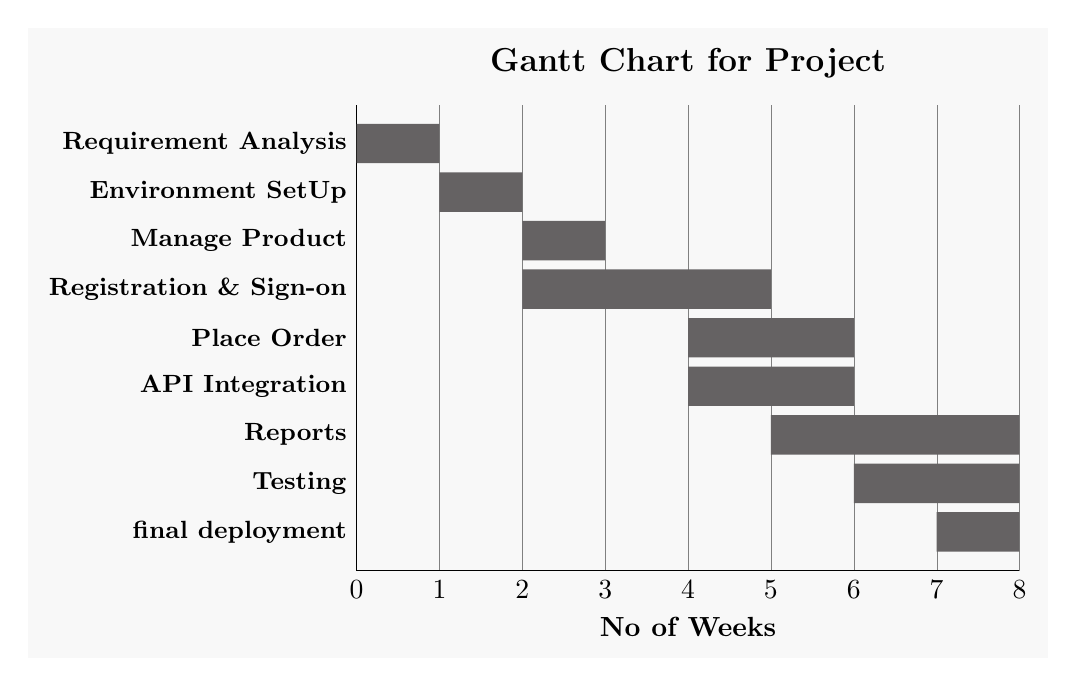
\begin{tikzpicture}[use background]
		
		\pgfplotstableread{ % Read the data into a table macro
			Label                                                      First   Second  
			{\small \textbf{final deployment}}                           7     1
			{\small \textbf{Testing}}                                    6     2
			{\small \textbf{Reports}}                                    5     3
			{\small \textbf{API Integration }}                           4     2
			{\small \textbf{Place Order}}                                4     2
			{\small \textbf{Registration \& Sign-on}}                    2     3
			{\small \textbf{Manage Product}}                             2     1
			{\small \textbf{Environment SetUp}}                          1     1
			{\small \textbf{Requirement Analysis}}                       0     1
		}\datatable
		
		\begin{axis}[
		xbar stacked,   % Stacked horizontal bars
		xmin=0,  xmax=8,       % Start x axis at 0
		title={\large \textbf {Gantt Chart for Project}},
		height=7.5cm, width=10cm,
		bar width=0.5cm,
		axis x line*=bottom,
		axis y line*=left,
		y axis line style={opacity=1},
		enlarge y limits=true,
		xmajorgrids={true},
		grid style={
			solid,
			ultra thin,
			gray
		},
		tick style={tickwidth=0cm,major tick length=0cm},
		xlabel={\textbf{No of Weeks }},
		ytick=data,     % Use as many tick labels as y coordinates
		yticklabels from table={\datatable}{Label}  % Get the labels from the Label column of the \datatable
		]
		\addplot [draw=none,fill=none] table [x=First, y expr=\coordindex] {\datatable};    % Plot the "First" column against the data index
		\addplot [draw=none,fill={levelfirst}]table [x=Second, y expr=\coordindex] {\datatable};
		
		
		\end{axis}
		

		\end{tikzpicture}
		

\end{center}
		
\noindent
These estimates may change nominally depending on the exact nature of detailed requirements.

\newpage



\subsection{Preliminary Product Description}
A VM Load Balancing Algorithm is selected and then implemented in Cloud Computing
environment using CloudSim toolkit, in java language. 
\\

In this algorithm, the VM assigns a varying (different) amount of the available processing power to the individual application services. These VMs are of different processing powers. The tasks/requests (application services) are assigned or allocated to the most powerful VM and then to the lowest and so on.
\\

Hence the given performance parameters such as response time and data processing time can be optimised, giving an efficient VM Load Balancing algorithm i.e. ‘Weighted Active Load Balancing Algorithm’ in the Cloud Computing environment.
\bigskip

\subsection{Conceptual Models}

\begin{figure}[H]
\centering
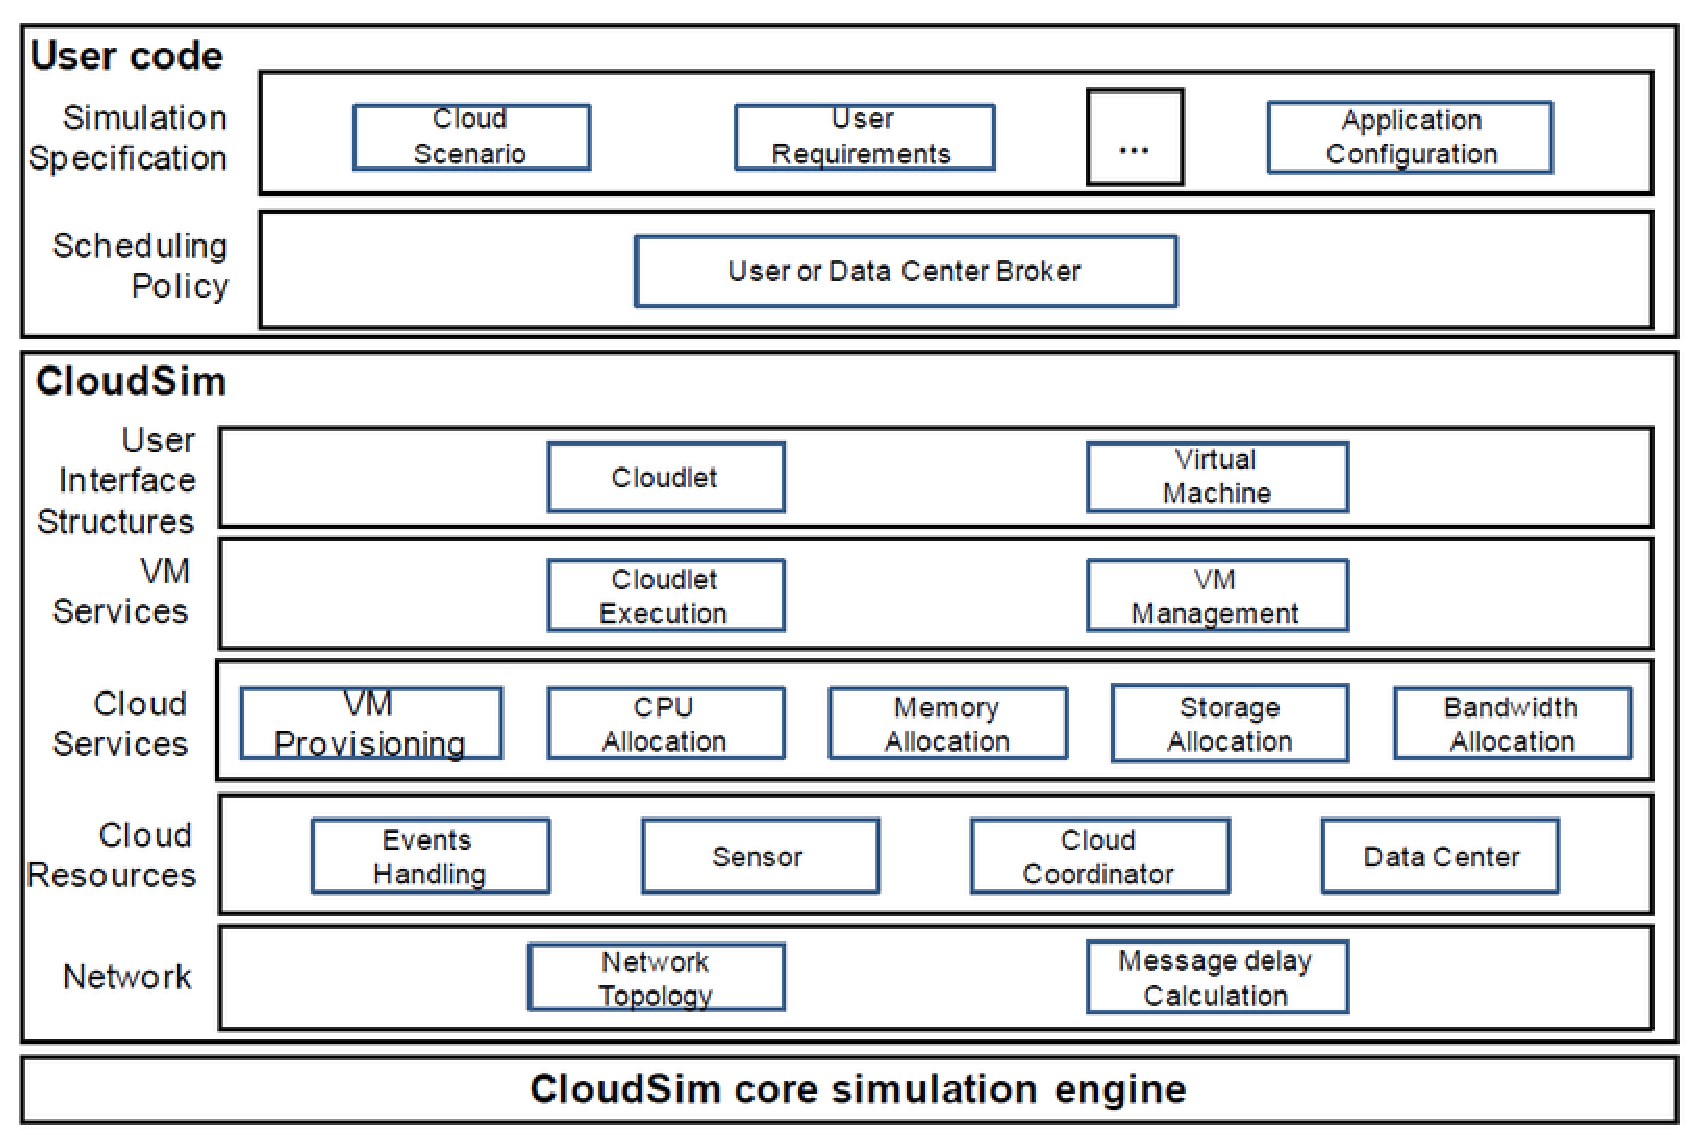
\includegraphics[ width=\textwidth , keepaspectratio ]{1.eps}\\[-1em]
\vspace{0.25cm}
\caption{Multi-Layer Design of CloudSim Framework}
\label{fig:1}
\end{figure}

Figure 1 shows the multilayer design of the cloudsim software framework and its architectural components. First layer is a simulation engine that supports several core functionalities, such as queuing and processing of events, creation of Cloud system entities (services, host, data center, broker, and virtual machines), communication between components, and management of the simulation clock. The CloudSim simulation layer provides support for modeling and simulation of virtualized Cloud-based data center environments including dedicated management interfaces for virtual machines (VMs), memory, storage, and bandwidth. The fundamental issues such as provisioning of hosts to VMs, managing application execution, and monitoring dynamic system state are handled by this layer. The top-most layer in the CloudSim stack is the User Code that exposes basic entities for hosts (number of machines, their specification and so on), applications (number of tasks and their requirements), VMs, number of users and their application types, and broker scheduling policies.
\bigskip

\begin{figure}[H]
\centering
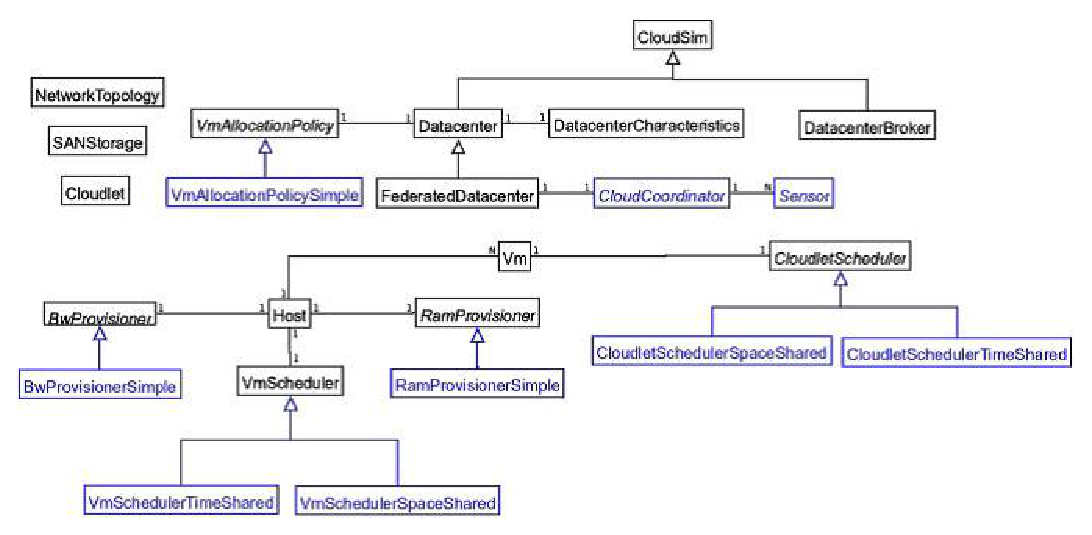
\includegraphics[ width=\textwidth , keepaspectratio ]{2.eps}\\[-1em]
\vspace{0.25cm}
\caption{Class Diagram of CloudSim -1}
\label{fig:2}
\end{figure}

\bigskip

\begin{figure}[H]
\centering
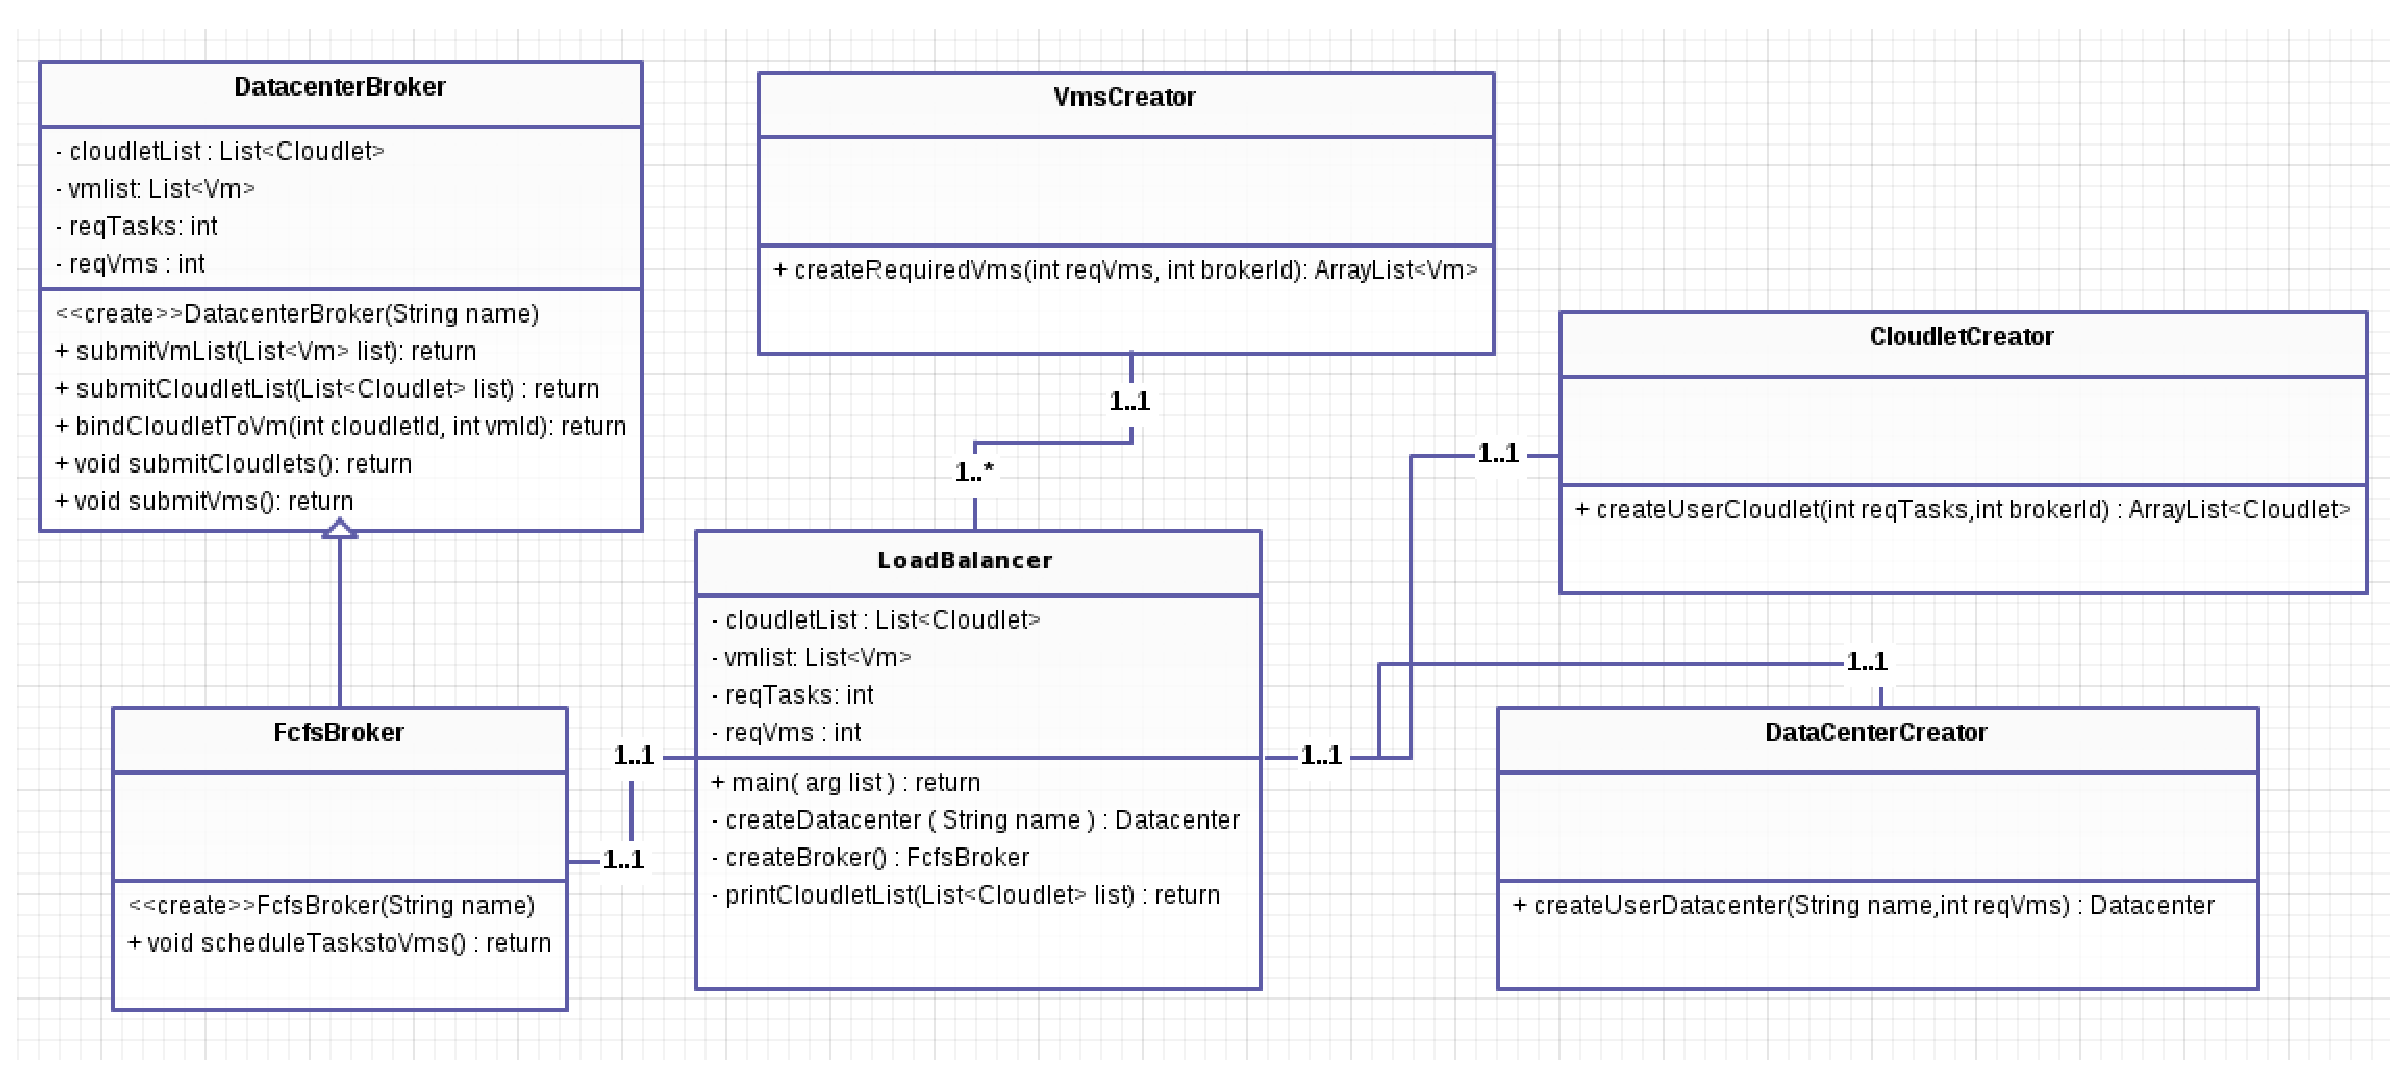
\includegraphics[ width=\textwidth , keepaspectratio ]{3.eps}\\[-1em]
\vspace{0.25cm}
\caption{Class Diagram of CloudSim -2}
\label{fig:3}
\end{figure}

Figure 2 \& 3 indicate the class diagram of CloudSim. These classes are building blocks of creating cloud applications and services. The existing classes and interfaces can be extended for experimenting and research solutions. Risk associated with the change of policy and technology is greatly simplified with simulation step with the cloudsim. Challenging and risk
oriented applications of cloud computing can be formulated and tested with the cloud environment provided by the cloudsim toolkit. The simulation and modeling environment provided by this is greatly helpful for the organizations seeking change with respect to the existing cloud services. Researchers can simulate and verify their research problem and accordingly take the corrective steps, if some issues remain unresolved.

\newpage 

\section{Scope of the Solution}
\subsubsection{Purpose}
This synopsis presents the scope to implement a VM load balancing algorithm: ``\textbf {Weighted Active Monitoring Load Balancing Algorithm}" to handle service request from user base
\\

\noindent
\subsubsection{Scope}
This Synopsis presents a background on Cloud Computing, introduces the Contemporary VM load balancers; and includes the selected VM load balancing algorithm for better response time and data processing time of cloudlets. This Synopsis also provides high level implementation details of the simulation and its setup.

\section{Analysis}

\section{Structure}

\section{Implementation of Security Mechanisms}

\section{Future Scope and further enhancement of Project}

\section{Bibliography}

\section{References}
\scriptsize {
[1] James Jasmin, Verma Bhupendra, "Efficient VM Load Balancing for a Cloud Computing Environment", International Journal on Computer Science and Engineering (IJCSE),ISSN : 0975-3397 Vol. 4 No. 09 Sep 2012, pp. 1658-1662
\\

\noindent
[2] Qi Zhang, Lu Cheng, Raouf Boutaba; Cloud computing: sate-of-art- and research challenges; Published online: 20\textsuperscript{th} April 2010, Copyright : The Brazillian Computer Society 2010.
\\

\noindent
[3]Michael Armbrust, Armando Fox, Rean Griffith, Anthony D.Joseph, Randy Katz; ‘Above the Clouds: A Berkeley View of Cloud Computing’; The Regents of the University of California, 2009 \\ 

\noindent
[4] Christ of Weinhardt, Benjamin Blau, Jochen Stober; ‘Cloud Computing- A Classification, Business Models, And Research Directions’, Business and Information System Engineering’. Vol 5. 2009, Pg 391-399 
\\

\noindent
[5] Rodrigo N.Calheiros, Rajiv Ranjan, Cesar A. F. De Rose, and Rajkumar Buyya; CloudSim: A Novel Framework for Modeling and Simulation of Cloud Computing Infrastructures and Services, Grid Computing and Distributed Systems (GRIDS) Laboratory, Dept. of Computer Science and Software Engineering, The University of Melbourne, Austrailia; Pontificial Catholic University of Rio Grande do Sul Porto Alegre, Brazil. {Rodrigo, rranjan, raj} @csse.unimelb.edu.au, cesar.derose@pucrs.br 
\\

\noindent
[6] Bhathiya Wickremasinghe, Rodrigo N. Calheiros, Rajkumar Buyya,“CloudAnalyst: A CloudSim-based Visual Modeller for Analysing Cloud Computing Environments and Applications”, 20-23, April 2010, pp. 446-452. 
\\

\noindent
[7] Cloud computing insights from 110 implementation projects; IBM Academy of TechnologyThought Leadership White Paper, October 2010. 
\\

\noindent
[8] IoannisPsoroulas,IoannisAnagnostopoulos,VassiliLoumos, Eleftherios Kayafas, “A Study of the Parameters Concerning Load Balancing Algorithms”, IJCSNS International Journal of Computer Science and Network Security, Vol. 7, No. 4, 2007, pp. 202-214 
\\

\noindent
[9] Sandeep Sharma, Sarabjit Singh, Meenakshi Sharma “Performance Analysis of Load Balancing Algorithms”, World Academy of Science, Engineering and Technology, 38, 2008 pp. 269- 27 
\\



\end{document}	
	









